\input{wg21common}

% Footnotes at bottom of page:
 \usepackage[bottom]{footmisc} 
 
 % Start sections at 0
 \setcounter{section}{-1}
 
 % pie charts
\usepackage{pgf-pie}  
 
 %%%%%%%%%%%%%%%%%%%%%%%%%%%%%%%%%%%%%%%%%%%%%%%%

%TABLE OF CONTENTS SETTINGS

\usepackage{titlesec}
\usepackage{tocloft}
 
% Custom ToC layout because the default sucks
\cftsetindents{section}{0in}{0.24in}
\cftsetindents{subsection}{0.24in}{0.34in}
\cftsetindents{subsubsection}{0.58in}{0.44in}
\cftsetindents{paragraph}{1.02in}{0.44in}

% Needed later to reduce the ToC depth mid document
\newcommand{\changelocaltocdepth}[1]{%
  \addtocontents{toc}{\protect\setcounter{tocdepth}{#1}}%
  \setcounter{tocdepth}{#1}%
}

\setcounter{tocdepth}{4}

 %%%%%%%%%%%%%%%%%%%%%%%%%%%%%%%%%%%%%%%%%%%%%%%%

\begin{document}
\title{\tcode{noexcept} policy for SD-9 (The Lakos Rule)}
\author{ Timur Doumler \small(\href{mailto:papers@timur.audio}{papers@timur.audio})  \\
John Lakos \small(\href{mailto:jlakos@bloomberg.net}{jlakos@bloomberg.net})
}
\date{}
\maketitle

\begin{tabular}{ll}
Document \#: & P3155R1 \\
Date: &2026-06-05 \\
Project: & Programming Language C++ \\
Audience: & LEWG
\end{tabular}

%%%%%%%%%%%%%%%%%%%%%%%%%%%%%%%%%%%%%%%%%%%%%

\begin{abstract}
This paper is a LEWG policy proposal as per \cite{SD-9}. It proposes to reconfirm the Lakos Rule (a function having a narrow contract should not be declared \tcode{noexcept}), a long-standing design principle of the C++ Standard Library, as an official LEWG design policy. We briefly summarise the rationale why the Lakos Rule is still an important and valuable design principle today -- and even more so now that contract assertions are in C++26. We present a quantitative study showing that the Lakos Rule is overwhelmingly followed in the existing C++ Standard Library specification, with exceptions to the rule being principled and clearly localised.
\end{abstract}

%%%%%%%%%%%%%%%%%%%%%%%%%%%%%%%%%%%%%%%%%%%%%

\tableofcontents*

%%%%%%%%%%%%%%%%%%%%%%%%%%%%%%%%%%%%%%%%%%%%%

\section*{Revision history}

Revision 1 (2026-06-04)
\begin{itemize}
\item Added prior art section
\item Expanded rationale
\item Rebased paper on C++26
\end{itemize}

Revision 0 (2024-04-16)
\begin{itemize}
\item Original version
\end{itemize}

\pagebreak

%%%%%%%%%%%%%%%%%%%%%%%%%%%%%%%%%%%%%%%%%%%%%

\section{Motivation and context}
\label{sec:intro}

A long-standing design principle in the C++ Standard Library is that a function having a narrow contract -- that is, a function specified to have \emph{preconditions} -- should not be declared \tcode{noexcept}, even if it is known to never throw an exception when called in-contract (i.e., without violating the preconditions). When we are convinced that a function having a narrow contract cannot throw when called in-contract, it should instead be specified as \emph{Throws: nothing}. This design principle is also known as the \emph{Lakos Rule}.

The Lakos Rule was first proposed in \cite{N3248} and adopted via \cite{N3279} in WG21 plenary (\cite{N3279}). An updated version of the rule was later codified into LEWG policy in \cite{P0884R0}; see \cite{O'Dwyer2018} for a more detailed summary.

\cite{P1656R2} proposed abandoning the Lakos Rule as a design principle for the C++ Standard Library. According to this paper, functions that are known to never throw an exception for a valid combination of input values and accessible state should always be declared \tcode{noexcept}, regardless of whether they have a wide or a narrow contract. Additionally, \cite{P2148R0} proposed adopting a set of design policies for the evolution of the C++ Standard Library that include moving away from the Lakos Rule.

While no policy to abandon the Lakos Rule has been formally adopted, LEWG nevertheless moved away from adhering to the Lakos Rule. LEWG leadership assumed the position that no formally adopted policy exists for how preconditions and \tcode{noexcept} should interact (\cite{P2920R0}); instead, we should consider each new proposal that contains narrow-contract functions on a case-by-case basis. This led to newer library facilities (e.g., \tcode{std::hive}) diverging from the Lakos Rule.

We believe that the Lakos Rule should remain a design principle for the C++ Standard Library. There are important engineering reasons why the Lakos Rule is still valid and useful today; abandoning it would inflict avoidable damage to the C++ language . To argue this case, we published two papers in the May 2023 mailing, \cite{P2831R0} and \cite{P2861R0}, and had planned to present them at the June 2023 meeting in Varna.

However, neither paper was scheduled for discussion in LEWG at the Varna meeting, nor at the following meeting in Kona in November 2023. Instead of considering our papers, LEWG has decided to first agree on a general process for adopting design policies for the C++ Standard Library. This has been done in \cite{SD-9}, with the actual policy-adoption process explained in \cite{P2267R1}.

According to this process, LEWG design policies should be adopted via \emph{policy papers}. Such policy papers must satisfy a number of requirements in order to be considered by LEWG. \cite{P2831R0} and \cite{P2861R0} have not been written with those requirements in mind, because they have been published before \cite{SD-9} was adopted, and were thus rendered ineligible for discussion in LEWG. The purpose of the present paper is to satisfy the requirements set out in \cite{P2267R1} and to serve as an ``envelope paper'' for \cite{P2831R0} and \cite{P2861R0} to make their content admissible for a \tcode{noexcept} policy discussion in LEWG, whenever this discussion is eventually scheduled.

Another paper relevant to this discussion is \cite{P3005R0}. Rather than proposing a concrete \tcode{noexcept} policy, it proposes a \emph{decision-making process} for how to agree on such a policy. The process outlined in \cite{P3005R0} involves systematic review of the entire design space: the paper considers seven possible candidate \tcode{noexcept} policies, six design questions that would need to be answered to choose one of those policies, and lists 20 design principles that can help us find the correct answers to those questions by following the \emph{principled-design} methodology proposed in \cite{P3004R0}. We believe that the process outlined in \cite{P3005R0} is an appropriate way to determine the best policy for the C++ Standard Library and establish consensus on that policy in LEWG. The present paper serves to aid this effort.

%%%%%%%%%%%%%%%%%%%%%%%%%%%%%%%%%%%%%%%%%%%%%

\section{Rationale}
\label{sec:rationale}

The rationale for retaining the Lakos Rule as a design policy has been thoroughly explored in our previous papers: \cite{P2831R0}, \cite{P2861R0}, and \cite{P3005R0}. We therefore refer the reader to those papers and references therein for details. Here, we provide only a brief summary of the most important engineering reasons to retain the Lakos Rule:

\begin{itemize}
\item \textbf{Contract widening.} Once a function with a narrow contract is specified as \tcode{noexcept}, its contract can never be widened to throw on what was previously a contract violation. For example, \tcode{std::vector::operator[]} could never be made backwards-compatibly bounds-checked with the behaviour of \tcode{std::vector::at} if it was \tcode{noexcept}. This is because \tcode{noexcept} is part of the type, part of the ABI, and directly observable via \tcode{operator noexcept}. Further, \tcode{noexcept} breaks Liskov substitutability — a bounds-checked subclass can no longer substitute for a narrow-contract base. On the other hand, \emph{Throws: Nothing} preserves the evolutionary freedom to widen the contract in a backwards-compatible and Liskov-substitutable way.
\item \textbf{Logical inconsistency.} Specifying a function as \tcode{noexcept} imposes a nothrow-guarantee over the entire syntactically valid input domain, contradicting the very definition of a narrow contract (the input domain is restricted, behaviour is undefined outside of it). \tcode{noexcept} thus effectively widens the contract in a specific way; the two concepts are inherently incompatible. Using \tcode{noexcept} on a narrow-contract function also contradicts the definition of undefined behaviour itself as behaviour on which the Standard imposes no restrictions. By imposing practical restrictions on UB, \tcode{noexcept} limits implementation freedom of how to mitigate it.
\item \textbf{Asymmetry of composition.} A C++ program adhering to the Lakos Rule can be written atop a library that does, but not atop one that does not. The C++ Standard Library is foundational, therefore it should follow the rule. Note that implementations remain free to strengthen \emph{Throws: nothing} to \tcode{noexcept} unilaterally. Therefore, retaining the Lakos Rule costs nothing -- on the other hand, abandoning it removes options irreversibly.
\item \textbf{Programmatic recovery.} There are many applications (e.g., in gaming, desktop publishing, host-plugin systems) for which throwing an exception on precondition failure and recovering programmatically is vastly preferable to terminating the program. However, a \tcode{noexcept} barrier turns any such throw into unconditional \tcode{std::terminate}. If the Lakos Rule is abandoned, such applications are permanently prevented from using any conforming Standard Library implementation. 
\item \textbf{Negative testing.} The cleanest, fastest, and only portable and scalable way to test that a precondition check actually fires is to throw from the assertion handler and catch it. However, this only works if functions with preconditions are not \tcode{noexcept}. All known alternatives (death tests via fork, clone, or spawn, \tcode{setjmp}/\tcode{longjmp}, child threads, signals, conditional-\tcode{noexcept} macros) are variously platform-specific and non-portable, orders of magnitude slower, UB-prone, or change the code under test (which is why libc++'s \tcode{_NOEXCEPT_DEBUG} experiment was abandoned as a ``horrible decision'').
\item \textbf{Foundational for Contracts.} The Lakos Rule is foundational for C++26 contract assertions, which were designed with the assumption that the Lakos Rule is an established design principle. C++26 allows a contract-violation handler to throw out of the function whose contract was violated, providing a standard way to implement programmatic recovery and negative testing. However, throwing contract-violation handlers do not work in the presence of \tcode{noexcept} barriers. C++26 contract assertions and \tcode{noexcept} are thus mutually exclusive if one wishes to use throwing contract-violation handlers. For a consistent language design, we need to either reinstate the Lakos Rule, or remove throwing contract-violation handlers. However, doing the latter has been rejected multiple times in EWG, whose position is clearly that throwing contract-violation handlers belong in the language.
\item \textbf{Misuse of \tcode{noexcept}.} There is no study showing measurable \emph{runtime} performance benefits through the use of \tcode{noexcept} on any modern platform. There is meeasurable impact on \emph{code size}, but the impact is minor, and for applications where code size really matters exceptions are typically disabled anyway. Merely documenting that a function cannot throw when called in-contract can be done through other, less risky and invasive means. The  genuine use case for \tcode{noexcept} -- and the only one for which it was originally designed -- is to enable an algorithm such as \tcode{std::vector::push_back} to choose a different, algorithmically more efficient code path for types that are nothrow-movable/copyable/swappable. When \tcode{noexcept} usage is limited to this use case, friction with the Lakos Rule (which was developed in concert with \tcode{noexcept} for C+11) disappears entirely.
\end{itemize}

%%%%%%%%%%%%%%%%%%%%%%%%%%%%%%%%%%%%%%%%%%%%%

\section{Prior art in the C++ Standard}
\label{sec:priorart}

The C++ Standard Library has been largely following the Lakos Rule as a design principle since \tcode{noexcept} was introduced in C++11 (\cite{N2855}, \cite{N3248}, \cite{N3279}), but exceptions do exist. We have conducted a detailed survey of narrow-contract functions across the entire current C++ working draft \cite{N5046} to both quantify and qualitatively describe these exceptions. We summarise the results of our survey in this section.

Counting both hardened and non-hardened preconditions, ignoring deprecated functions in Annex D, and properly accounting for member functions of concrete container types that are described in generic clauses such as [sequence.reqmts], we counted 1284 narrow-contract functions in the C++ Standard library (out of 7165 total, i.e. 17.9\%). Out of these 1284 narrow-contract functions:
\begin{itemize}
\item 1053 functions (82.0\%) are not \tcode{noexcept}, i.e. they follow the Lakos Rule unconditionally. 
\item 204 functions (15.9\%) are \tcode{noexcept}, i.e. they violate the Lakos Rule. 
\item 27 functions (2.1\%) are \emph{conditionally} \tcode{noexcept}. 
\end {itemize}
A pie chart visualising this distribution is shown in Figure \ref{fig:piechart}. 

%~~~~~~~~~~~~~~~~~~~~~~~~~~~~~~~~~~~~~~~~~~~~~~~~~~~~~~~~~~~~~~~~~~~
\vspace{5mm} % added manually to create enough space between text and piechart
\begin{figure}[b!]
    \centering
    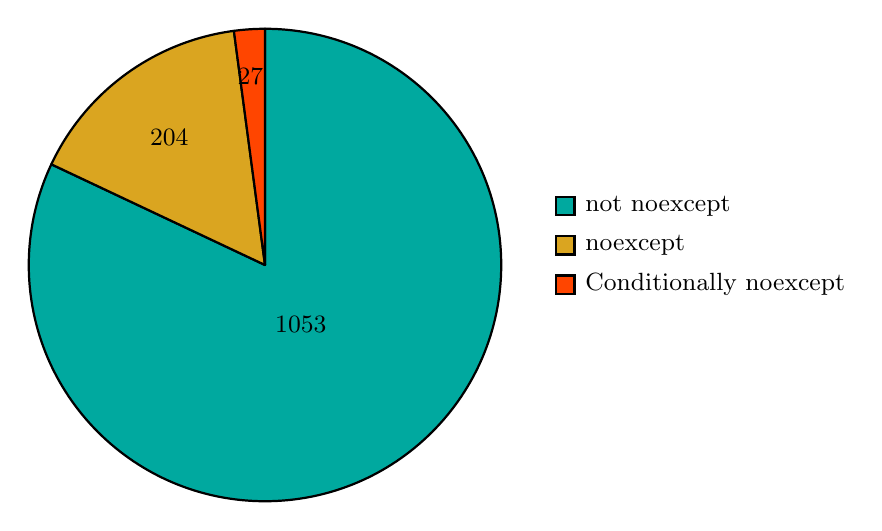
\begin{tikzpicture}
        \pie[text=legend, 
               radius=3, 
               rotate=90,
               change direction,
               color={Emerald, Goldenrod, OrangeRed},
               sum=auto,
               after number = \,,   % keeps numbers tidy (adds thin space)
               /tikz/nodes={font=\small} % tweak font size if needed
            ]
            {1053/not \tcode{noexcept}, 204/\tcode{noexcept}, 27/Conditionally \tcode{noexcept}}
    \end{tikzpicture}
    \caption{\tcode{noexcept}-ness of narrow-contract Standard Library functions across the current C++ working draft}
    \label{fig:piechart}
\end{figure}
%~~~~~~~~~~~~~~~~~~~~~~~~~~~~~~~~~~~~~~~~~~~~~~~~~~~~~~~~~~~~~~~~~~~

Violations of the Lakos Rule are not random, but principled (at least, before C++26). Almost all narrow-contract functions that are conditionally \tcode{noexcept} are clearly localised in the following clusters, ordered from most to least common:
\begin{itemize}
\item Dereferencing observers and accessors in smart pointers, \tcode{std::optional},  \tcode{std::expected}, \tcode{std::span}, and \tcode{std::mdspan};
\item Low-level, concurrency-related facilities such as \tcode{std::atomic}, \tcode{std::atomic_ref}, hazard pointers, RCU;
\item Deallocation functions such as \tcode{operator delete(void*)}, which are forbidden from throwing by core language rules;
\item Functions that cannot throw by the very nature of their operation, even if called out-of-contract, such as \tcode{std::launder} and \tcode{std::start_lifetime_as};
\item Lakos Rule violations in facilities newly introduced in C++26, such as \tcode{std::hive} and \tcode{std::saturating_div}.
\end{itemize}
The first and fourth clusters are deliberate, well-motivated divergences from the \tcode{noexcept} policy established via \cite{P0884R0}; the second and third are in line with the policy; the last one indicates recent divergence in the absence of a policy.

Conditionally-\tcode{noexcept} functions with narrow contracts are few. They are localised in the following two clusters:
\begin{itemize}
\item Swap and move operations: \tcode{std::swap}, member \tcode{swap}, \mbox{\tcode{iter_swap}}, \tcode{iter_move}, move-assign operators;
\item Forwarding \tcode{operator()(Args...)} in function wrappers \tcode{std::move_only_function} and \mbox{\tcode{std::copyable_function}}.
\end{itemize}
In all of the above cases, the throwing behaviour tracks that of a template parameter, in line with the policy in \cite{P0884R0}. This is a narrow, well-defined idiom that has been explicitly designed with the Lakos Rule in mind, carving out precise exceptions to the rule where algorithmically necessary.

Apart from the above clusters and a small handful of isolated cases, the C++ Standard Library consistently adheres to the Lakos Rule. Many popular and widely used C++ Standard Library facilities adhere to the Lakos Rule \emph{without any exceptions}: all containers introduced before C++26 (\tcode{std::vector}, \tcode{std::array}, associative containers), all algorithms introduced before C++26, as well as \tcode{std::variant}, \tcode{std::pair}, \tcode{std::tuple},  \tcode{std::mutex}, and \tcode{std::chrono}. Other popular facilities such as \tcode{std::thread} are entirely wide-contract so the question does not arise.

The use of  the ``\emph{Throws:} Nothing'' specification idiom  is widespread, but not rigorous -- sometimes the ``\emph{Throws:}'' clause is missing even if a non-\tcode{noexcept} function will not throw in-contract, such as for \tcode{operator[](size_t)} for array \tcode{std::unique_ptr}.

Our analysis demonstrates that the Lakos Rule is the norm in the C++ Standard Library today. Therefore, reinstating the Lakos Rule as official LEWG policy is the only choice consistent with the status quo in the C++ Standard Library specification.

%%%%%%%%%%%%%%%%%%%%%%%%%%%%%%%%%%%%%%%%%%%%%

\section{Status quo in the wider C++ community}
\label{sec:statusquo}

Community surveys such as the JetBrains Developer Ecosystem survey, the Meeting C++ Community Survey, and the Standard C++ Foundation's Annual C++ Developer Survey consistently show that about half of C++ developers work on codebases where exceptions are either partially or completely banned from use; for the latter in particular, the \tcode{noexcept} policy is of little relevance.

Codebases that \emph{do} use exceptions fall into different camps. Many C++ libraries generously sprinkle \tcode{noexcept} all over their code, while codebases relying on techniques like exception-based recovery and negative testing adhere to the Lakos Rule (see \cite{P2831R0} for case studies of several companies with such codebases, across different industries).

Quantifying the relative size of these camps is difficult and we did not attempt to do so for this paper. However, we expect the use of these techniques to become significantly more widespread with the adoption of C++26 contract assertions, which permit attaching a throwing contract-violation handler as a \emph{standard}, portable mechanism for exception-based recovery from assertion failures.

The three major implementations of the C++ Standard Library (GCC, Clang, and Microsoft) do not use the Lakos Rule and generally tighten \emph{Throws: nothing} to \tcode{noexcept}, making them incompatible with these techniques; other implementations of the Standard Library, or parts of it, such as Bloomberg's BDE, follow the Lakos Rule and make extensive use of exception-based recovery and negative testing.

%%%%%%%%%%%%%%%%%%%%%%%%%%%%%%%%%%%%%%%%%%%%%

\section{Proposed policy}
\label{sec:policy}

We propose to retain the \tcode{noexcept} policy that we have already had for a long time and that the vast majority of the C++ Standard Library follows today: the one described in \cite{P0884R0}, refining the original formulation in \cite{N3279}. This policy consists of the following rules, which includes the Lakos Rule:
\begin{enumerate}[label=\alph*)]
\item No library destructor should throw. They shall use the implicitly supplied (nonthrowing)
exception specification.
\item If a library function has a wide contract (i.e., does not specify undefined behavior due to a precondition), it should be marked as unconditionally \tcode{noexcept} if it cannot throw; if it has a narrow contract, it should be specified as \emph{Throws: Nothing} if it cannot throw when called in-contract.
\item If a library swap function, move-constructor, or move-assignment operator is
conditionally-wide (i.e. can be proven to not throw by applying the \tcode{noexcept} operator)
then it should be marked as conditionally \tcode{noexcept}.
\item If a library type has wrapping semantics to transparently provide the same behavior as
the underlying type, then default constructor, copy constructor, and copy-assigment
operator should be marked as conditionally \tcode{noexcept} matching the underlying exception
specification.
\item No other function should use a conditional \tcode{noexcept} specification.
\item Library functions designed for compatibility with C code (such as the atomics facility)
may be marked as unconditionally \tcode{noexcept}. 
\end{enumerate}
Note that this set of rules corresponds to Policy C in \cite{P3005R0}, which considers seven possible \tcode{noexcept} policies B-H in addition to the null policy A (``no policy'').

%%%%%%%%%%%%%%%%%%%%%%%%%%%%%%%%%%%%%%%%%%%%%

\section{Rationale for adopting a policy}
\label{sec:rationale_adopt}

The question of which \tcode{noexcept} policy the C++ Standard Library should follow has been a hotly debated topic in recent years, taking up a considerable amount of committee time. Equally, per-proposal per-function re-litigation of \tcode{noexcept}-ness -- required in the absence of any agreed-upon policy, which seems to be the status quo -- is also an inefficient use of committee time.

While no official policy exists, the C++ Standard Library continues to drift apart on this question, with the bulk of it adhering to the Lakos Rule as originally intended but newer (C++26) facilities departing from it. This creates inconsistencies and growing technical debt that will need to be retroactively fixed via Defect Reports once we have an agreed-upon policy, which will consume even more committee time.

For all of the above reasons, we should put this debate to rest and adopt a \tcode{noexcept} policy as soon as possible. 

%%%%%%%%%%%%%%%%%%%%%%%%%%%%%%%%%%%%%%%%%%%%%

\section{Proposed wording}
\label{sec:wording}

Append to ``List of Standard Library Policies'' section of SD-9 the items a) -- f) enumerated in Section \ref{sec:policy} above.

%%%%%%%%%%%%%%%%%%%%%%%%%%%%%%%%%%%%%%%%%%%%%


\section*{Disclaimer}
The quantitative survey of Lakos Rule adherence across the entire C++ working draft has been performed with the help of an LLM. The exact prompts used for this survey and their full output are available from the authors upon request.

\section*{Acknowledgements}
We wish to express our gratitude to the late Ed Catmur, co-author of \cite{P2831R0}, for his valuable contributions to this effort until his tragic death during a fell run on 31 December 2023.

%%%%%%%%%%%%%%%%%%%%%%%%%%%%%%%%%%%%%%%%%%%%%

\renewcommand{\bibname}{References}
\bibliographystyle{abstract}
\bibliography{ref}

\end{document}
